\usefont{OT1}{phv}{m}{n}

% Parler des produits d'abord. 
% Parler de Bob Booking d'abord, puis les autres produits. 

\chapter{Introduction}

\section{La société}

\subsection{Historique}
Basée à Bordeaux, la société \textbf{Bob el web} est une SAS de 10 salariés créée en 2006 par Jean-Luc Mirebeau et Fred Wolf.
L'activité principale de la société consiste à développer et commercialiser des logiciel de gestion de type CRM (customer relationship management). 

L'expérience de M. Mirebeau dans le monde du spectacle, étant lui-même anciennement "tourneur", lui a permis d’établir le constat que l'organisation d'événements pourrait être plus rapide si les outils informatiques utilisés étaient réunis au sein d'une même plateforme. Il s'est donc lancé dans la création du logiciel Bob Booking.


\subsection{Activité}

L'activité de l'entreprise est centrée autour de la vente de logiciel CRM en B2B (business to business) à destination des professionnels du spectacle en particulier les "tourneur".


\subsubsection{Qu'est-ce qu'un tourneur ?}
Le tourneur imagine, propose et gère une série de spectacles d'un artiste sur un territoire, auprès de lieux de diffusion et sur une période donnée. Il coordonne les efforts de différents programmateurs et promoteurs locaux. Il peut être producteur du spectacle et directement travailler avec les artistes ou bien représenter d'autres producteurs auprès des diffuseurs. Il administre une tournée, y compris les aspects logistiques, techniques et financiers. Il communique auprès de partenaires variés pour valoriser les projets qu'il présente et commercialise des représentations.

\subsubsection{Produits}
Il existe actuellement plusieurs produits proposés et commercialisés par l'entreprise sous forme d'application web (accessible depuis internet et par le biais d'un abonnement).

Chaque produit a des fonctionnalités différentes et vise une cible différente correspondant à un métier spécifique du monde du spectacle.

\newpage


\subsubsection{Bob Booking}

\begin{figure}[h!]
	\centering
	
\includegraphics[width=0.2\textwidth]{assets/booking.png}
\end{figure}


Bob Booking représente le produit ayant des parts de marché élevées sur un marché en faible croissance. 
Ce produit exige peu d'investissements de la part de la société et dégage des flux financiers importants.
C'est la véritable \textbf{\gls{vache} de l'entreprise} 
\jumpTwo
Bob Booking est un outil de communication et de relation commerciale où tout est conçu pour agir efficacement sur l’ensemble des fichier de contacts client.
C’est aussi un outil performant de booking.
Permettant de gérer les tournées et prévisions budgétaires qui s’affichent en temps réel, exportables sous tout types de formats.

C’est enfin un outil d’administration et de régie avec un cycle automatisé de confirmation / contrat / facture, la gestion des équipes sur la route et des VHR.



\begin{figure}[h!]
    \centering
    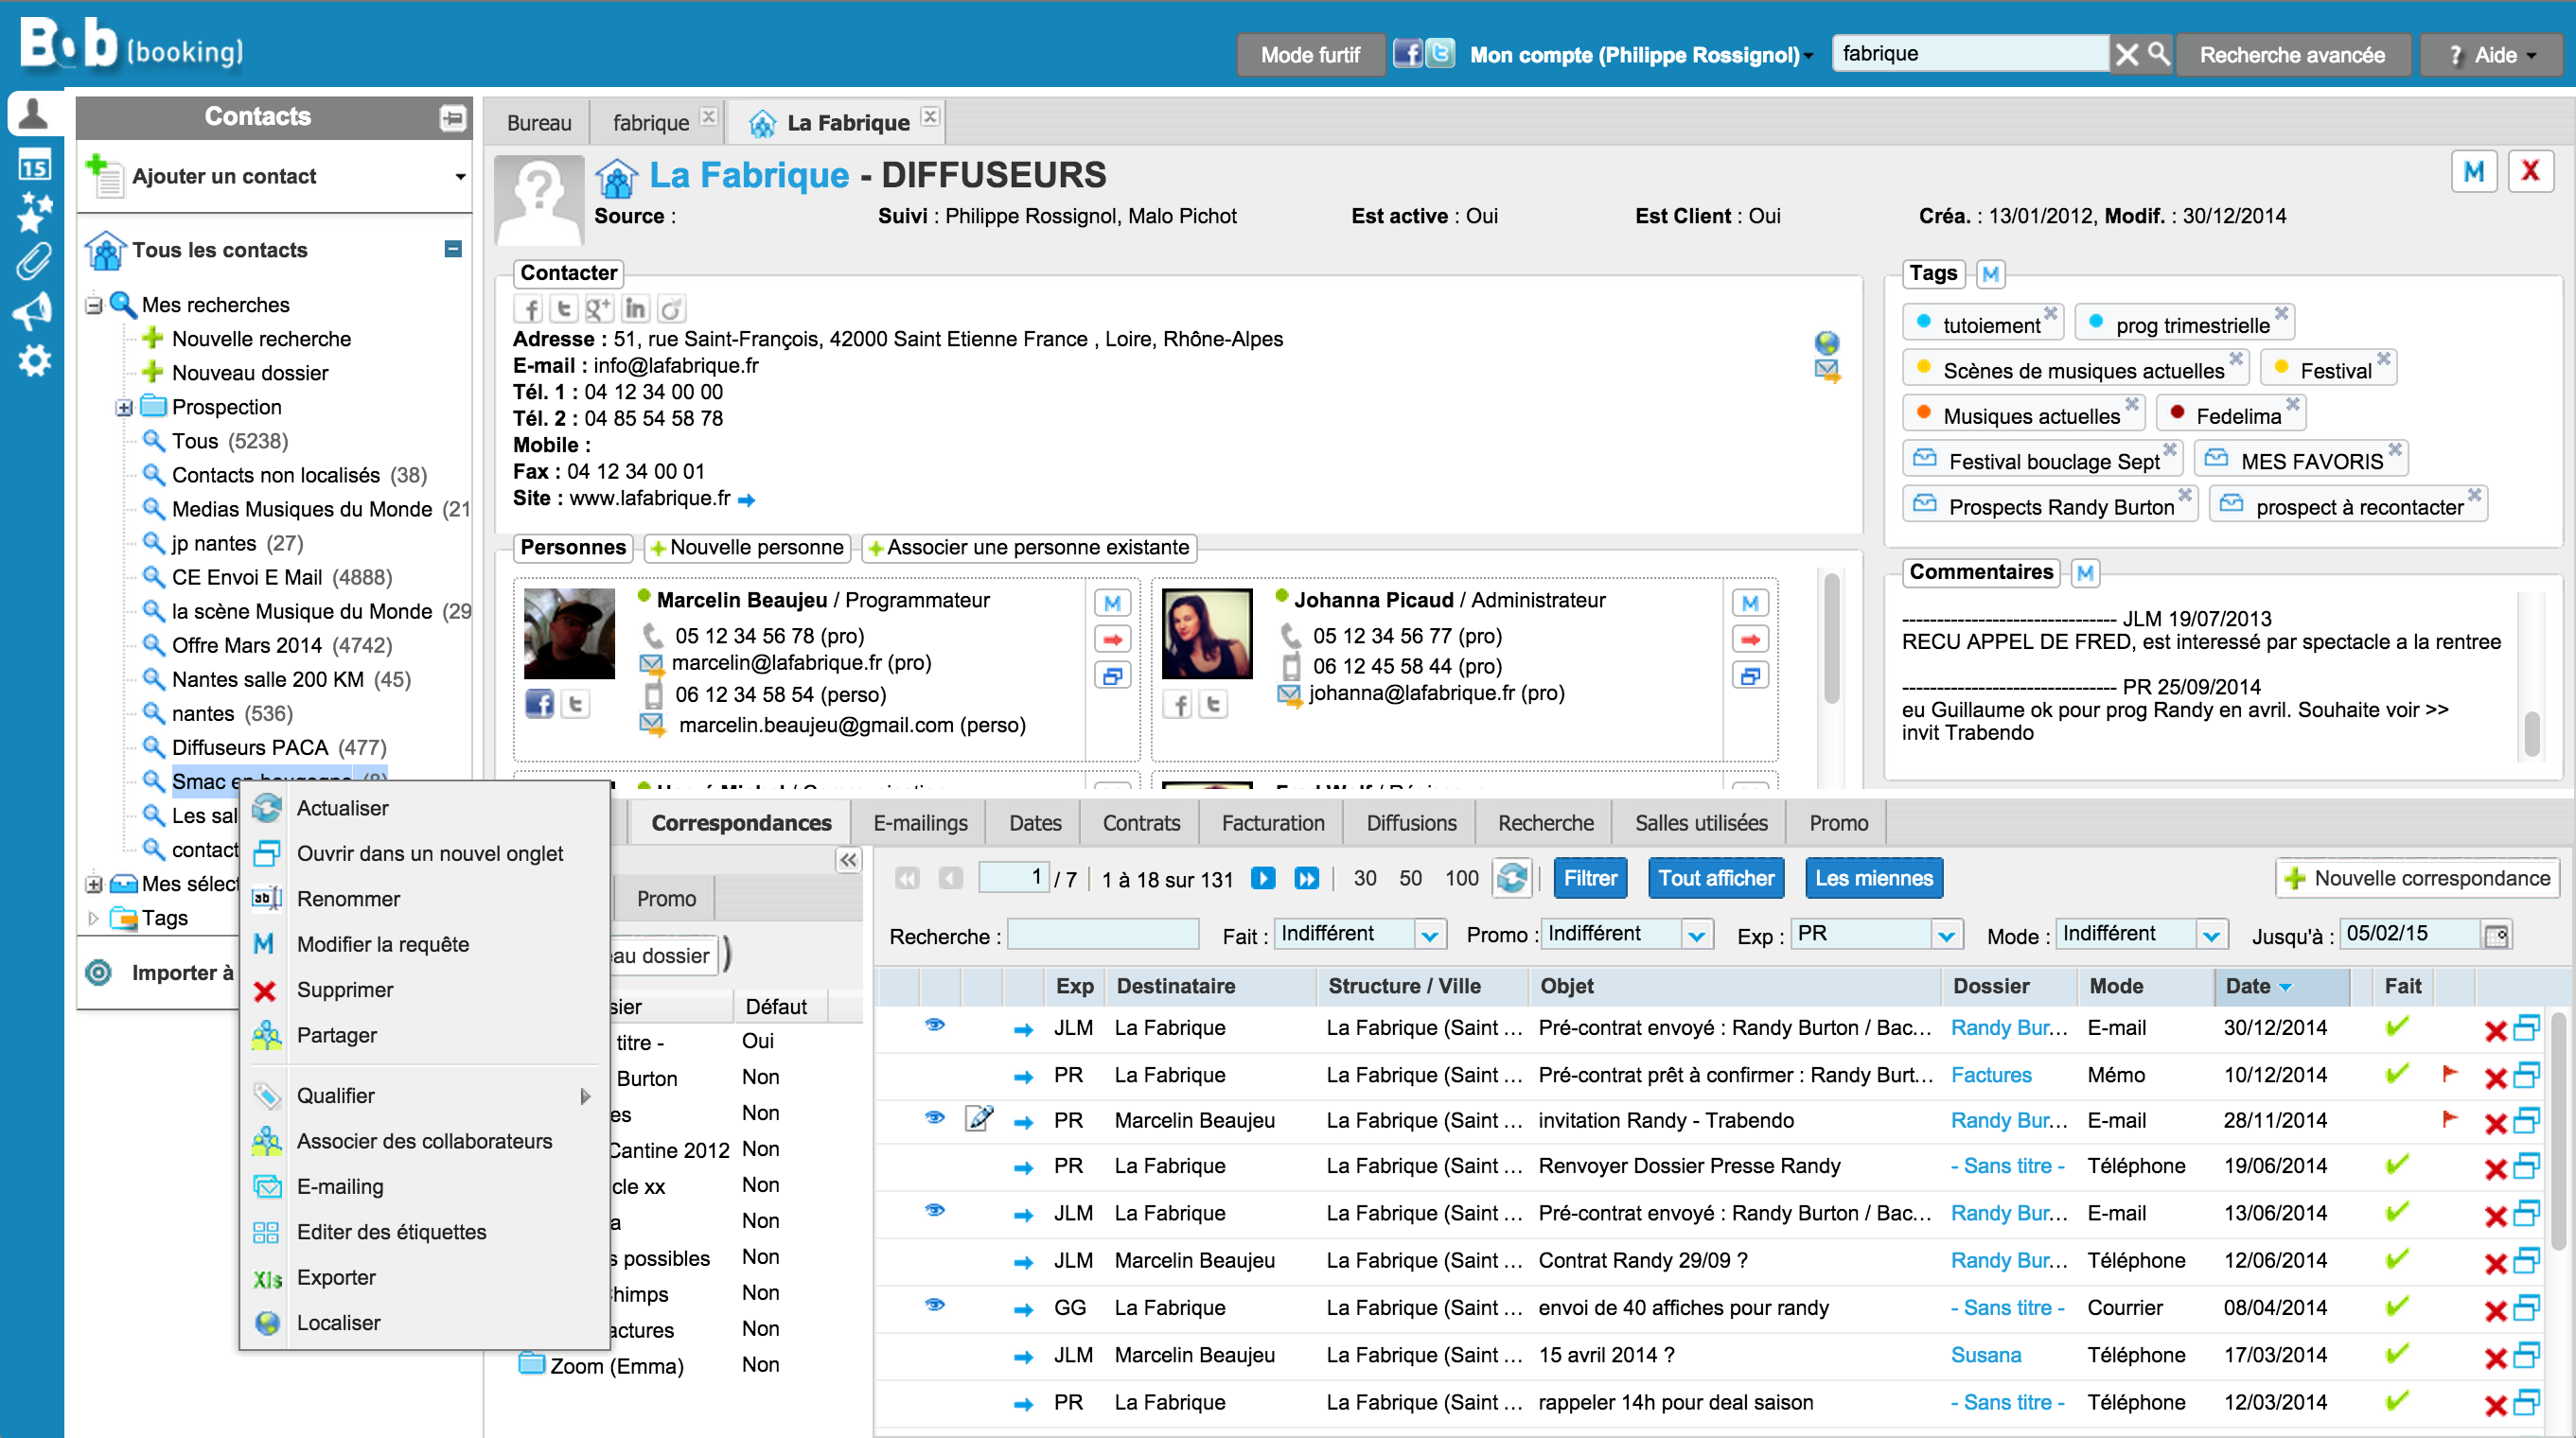
\includegraphics[width=1\textwidth]{assets/bob_screenshot.png}
    \caption{Capture d'écran du logiciel Bob}
    \label{fig:my_label}
\end{figure}

Le logiciel propose ainsi de multiples fonctionnalités

\begin{itemize}
    \item Import et gestion de contact
    \item Recherches avancées à travers l'ensemble des contacts. 
    \item Dossiers de relance et historiques
    \item Envoi d'email
    \item Gestion des campagnes d'emailing ciblés et tracés.
    \item Gestion electronique des documents
    \item Agenda Collaboratif
    \item Comptes, gestions des permissions
    \item etc.
\end{itemize}

Les produits suivants, sont des versions différentes du produit Bob Booking, adapté en fonction des besoins. 


\begin{minipage}{0.3\textwidth}
	\begin{figure}[H]
		\centering
		
\includegraphics[width=0.8\textwidth]{assets/express.png}
    \end{figure}
\end{minipage}%
\begin{minipage}{0.6\textwidth}

% Parti du constat que des les petites structures ne veulent pas toutes les fonctionnalités 
% proposés par Bob. C'est une version minimale 

C'est une version minimale de Bob Booking comprennant uniquement les fonctionnalités principales. 

Bob Express est réservé aux structures émergentes (indépendants, auto-entrepreneurs...) et aux entreprises de l’économie sociale et solidaire.
\end{minipage}

\vspace{5mm}


\begin{minipage}{0.3\textwidth}
	\begin{figure}[H]
		\centering
		
\includegraphics[width=0.8\textwidth]{assets/festival.png}
    \end{figure}
\end{minipage}%
\begin{minipage}{0.6\textwidth}
Bob Lieu \& Festival a été conçu pour centraliser, enrichir et partager toutes les informations et actions nécessaires à la gestion d’événements culturels.

Scénarios de programmation, communication massive vers les fichiers publics, gestion multi-lieux et multi-projets, tâches techniques, affectation des bénévoles ou des intermittents, horaires et ressources techniques…
\end{minipage}

\begin{figure}[h!]
    \centering
    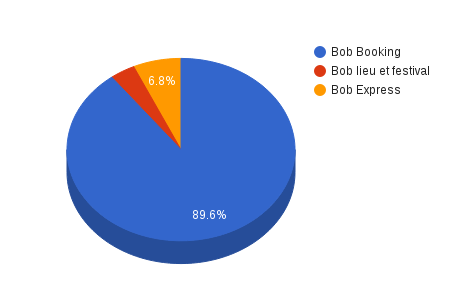
\includegraphics[width=0.8\textwidth]{assets/repartition_client.png}
    \caption{Répartition des clients sur les produits}
    \label{fig:my_label}
\end{figure}

\newpage


\subsection{Purple Base}

Depuis quelques mois l'entreprise travaille à la création d'un nouveau logiciel (dont la sortie est prévu à la fin de l'année 2015), appelée Purple Base. 

\subsubsection{Contexte}
 L'entreprise se retrouve face à la situation ou Bob Booking, a saturé le marché du booking avec environ 50\% de \gls{part de marche en valeur}.
Il est urgent pour l'entreprise de trouver un nouveau relai de croissance. 

En ciblant une nouvelle clientèle : les indépendants, les groupes auto-diffusés.
En proposant avec des technologie de pointes, la mise à disposition d'informations commerciale sur le secteur du booking.

Purple Base est un référentiel de données commerciale du secteur musical,  mis à jour en permanence. 
En présentant une interface nouvelle centralisant les informations des petites structures, l'entreprise souhaite révolutionner le booking indépendant et prendre un nouveau départ. 


% Présentation de purple base, pourquoi ? 
% Réponses de JLM
% Evol du CA -> DONE 
% Présentation de Purple Base 
%Pourquoi ? 
%2 objectifs. 
%- Technologique ; contribuer à un renouveau de l'entreprise en réecrivant la technologie associé (les technologie utilisés se basent sur des techno assez vieilles). 
%- Cible différente (Bto2), petit produit pour groupe auto-diffusé
%--> Offre révolutionner le booking indé. 
%- L'entreprise à une cible + large et veut tailler des part de marchés à des concurrents. 
%C'est quoi ? 
%Référentiel de données, mit à jour en permanence avec les meilleurs données du secteur, une interface toute nouvelle, permettant d'avoir tout au même endroit.
%Comment PB est venu à l'idée ? 
%- Bob booking a saturé le marché du booking avec + de 40/50 \% de PDM en valeur. 
%ainsi il était nécessaire d'avoir un relai de croissance. 
%- Ainsi PB a été l'occasion de choper d'autres part de marché et tout refaire technologiquement

\subsubsection{Architecture}

D'un point de vue architecture, Purple Base se base sur l'application Bob Booking (par le biais d'une Api) pour réaliser les actions sur le serveur. 

Purple Base ayant des fonctionnalités commune avec les logiciels déjà développés, le but étant de se baser sur Bob Booking pour ne pas tout refaire depuis le début et donc gagner du temps. 

\begin{figure}[h!]
\centering
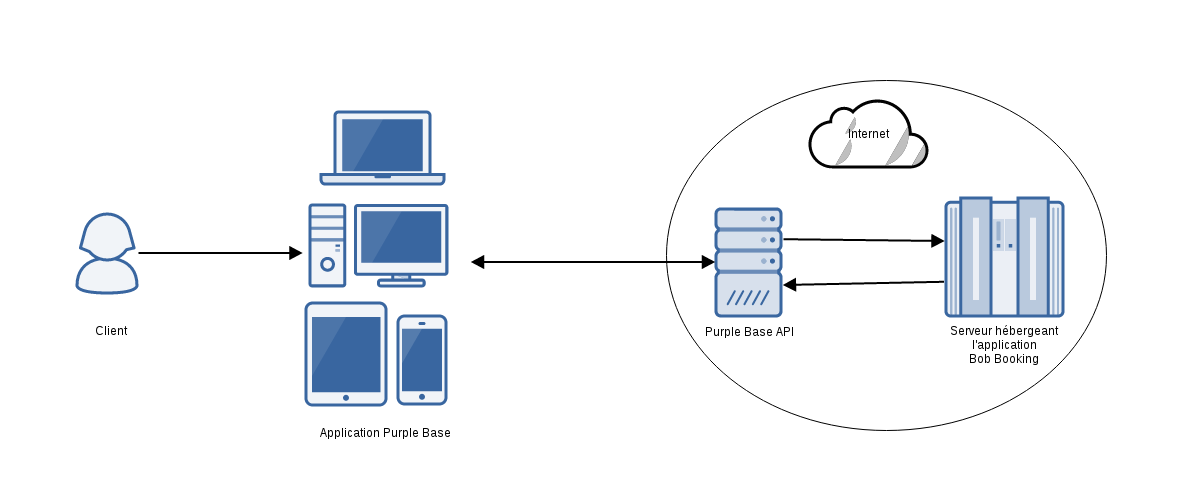
\includegraphics[width=1\textwidth]{assets/archi_pb.png}
\caption{Représentation de l'architecture du logiciel}
\label{fig:my_label}
\end{figure}


\subsubsection{Chiffre d'affaire}

\begin{figure}[h!]
\centering
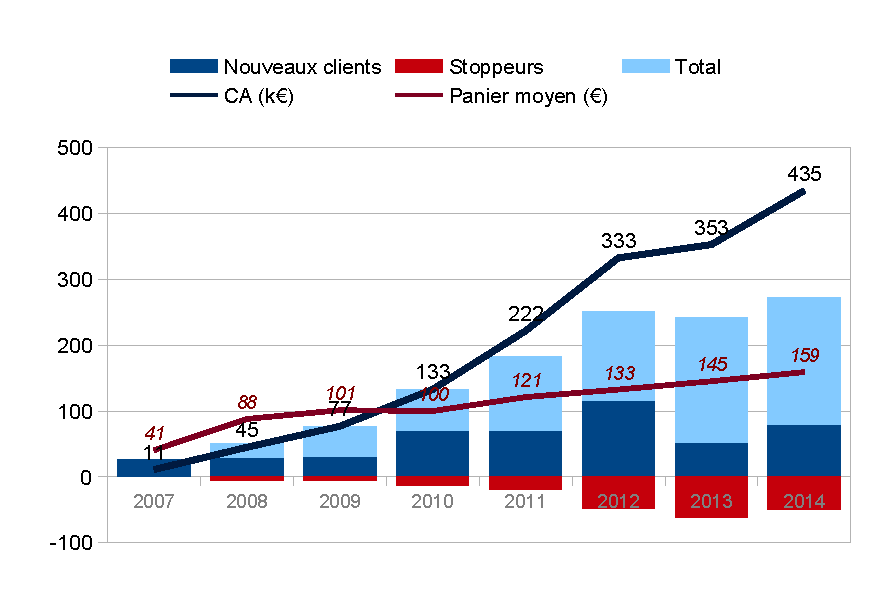
\includegraphics[width=0.8\textwidth]{assets/evol_ca_bob.pdf}
\caption{Evolution du CA depuis la création de l'entreprise}
\label{fig:my_label}
\end{figure}

\subsubsection{Répartition du chiffre d'affaire en 2014}

\begin{minipage}{.6\textwidth}
    \begin{description}
        \item[Prestation de coproduction]
        {5\% du CA est représenté par ces coproduction. 
        Ce sont des prestations que l'entreprise réalise à la demande des clients. Une nouvelle         fonctionnalité qu'un client voudrait avoir dans sont application.
        }
        \item[Vente crédit d'emailing]
        {9\% du CA est représenté par la vente de crédit d'emailing. 
        L'application Bob Booking permet de gérer des campagnes d'emailing. 
        Chaque email envoyé depuis l'application nécessite du crédit. 1 crédit = 1 destinaire d'une campagne. 
        Par exemple pour envoyer 10 campagne à 2000 destinataires, nécessitera 20 000 crédits. 
        }
        \item[Formation client]
        {18\% du CA est représenté par des formations sur les différents logiciels proposés. 
        }
        \item[Nouveaux abonnements]
        {
        Durant l'année 2014, 11\% du CA est représenté par de nouveaux abonnements. Des nouveaux         clients qui ont souscrit pour un Bob Booking ou Express, etc. 
        }
        \item[Abonnements]
        {
        57\% du chiffre d'affaire est représenté par les abonnements des anciens clients. 
        }
        
    \end{description}
\end{minipage}% This must go next to `\end{minipage}`
\begin{minipage}{1\textwidth}
    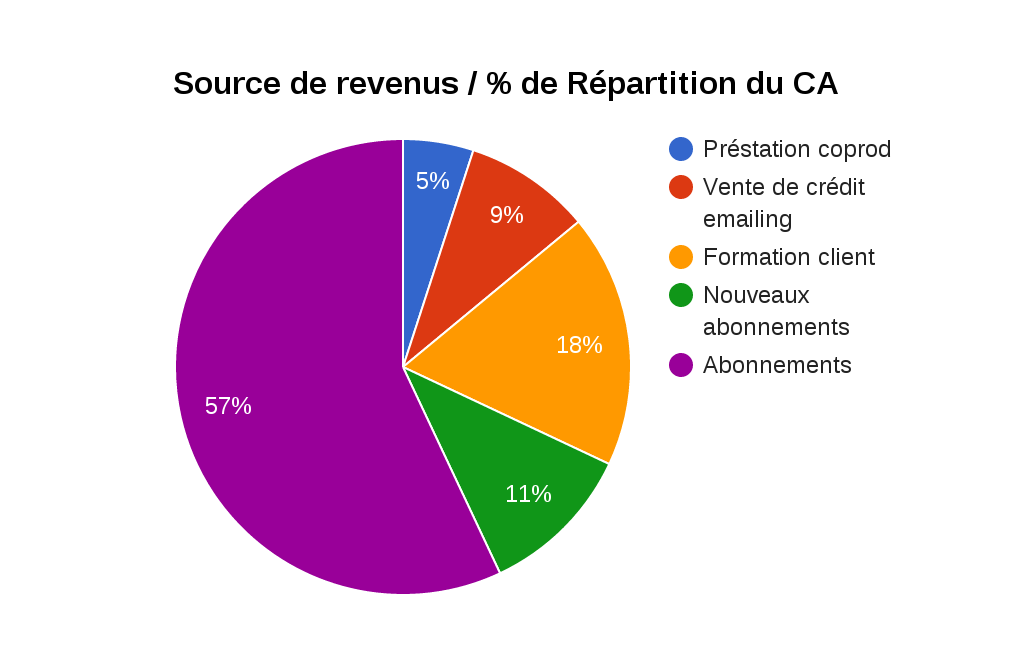
\includegraphics[width=0.65\textwidth]{assets/repartition_ca.png}
\end{minipage}



